\documentclass[a4paper]{usiinfbachelorproject}

\captionsetup{labelfont={bf}}
%%%%%%%%%%%%%%%%%%%%%%%%%%%% PACKAGES %%%%%%%%%%%%%%%%%%%%%%%%%%%%%
\usepackage{float}
\usepackage{amsmath}

%%% Main Body %%%

\author{Sasha Toscano}

\title{\textbf{Understanding arbitrary code
execution}}
\subtitle{A case study on Pokémon Emerald}
\versiondate{\today}

\begin{committee}
%With more than 1 advisor an error is raised...: only 1 advisor is allowed!
\advisor[Universit\`a della Svizzera Italiana, Switzerland]{ }{Carlo Alberto}{Furia}
%You can comment out  these lines if you don't have any assistant
\coadvisor[Universit\`a della Svizzera Italiana, Switzerland]{ }{Marc}{Langheinrich}

\end{committee}

\abstract { Abstract goes here ...
You may include up to six keywords or phrases. Keywords should be separated with semicolons. 
\\
\textbf{Keywords}:

}
\begin{document}
\maketitle
\tableofcontents\newpage
%\listoffigures\newpage

\section{\textbf{Introduction}}
In the world of software, security is one of the most critical concepts as it is the foundation of trust in the software we use every day. Let it be something as simple as our browser remembering our passwords, or as complex as a bank's online banking system, we need to be able to trust that the software we use is secure and that our data is safe and well protected. This is especially important in this day and age where we rely on these types of software for everything: from communication, to banking, and even to entertainment.

The software we use is often complex and interconnected, making it difficult to ensure what is secure and what isn't. In many cases, these programs are often developed quickly and with limited resources, and as a result, security is often an afterthought in the development process, leading to oversights or the introduction of vulnerabilities that can be exploited by attackers.

One of the most common types of these vulnerabilities is arbitrary code execution (ACE), which allows a malicious user the ability to execute some arbitrary code on a target system or on a specific application. This can happen because software or computer systems in general are not capable of differentiating between some generic text and actual commands, without some proper protections put in place.

This then becomes a significantly serious issue as it can lead to unauthorized access to sensitive information, data loss, and even complete system compromise. These types of ACE vulnerabilities can be found in a wide range of software: including operating systems, web applications, and even video games. In fact, some very dangerous ACE vulnerabilities have been found in video games like \textit{Super Mario World}, where they have been used to allow users to literally "program" new games into the system mid-run.

In this thesis, we will explore the concept of ACE in detail, using a case study of the game \textit{Pokémon Emerald (2004)} to illustrate how these vulnerabilities can be exploited and to understand the importance of creating state of the art protections against this type of attacks. After which we will discuss the state of the art in ACE vulnerabilities and how they can be mitigated. We will also look at some of the most common techniques used to protect against these vulnerabilities, and how they can be prevented.

\section{\textbf{Arbitrary code execution}}
I'd like to start with a simple explanation of what arbitrary code execution (ACE in short) is: \textit{updog}. And what is updog, you may ask? \textit{Not much, what's up with you?}.

\begin{figure}[h!]
	\center{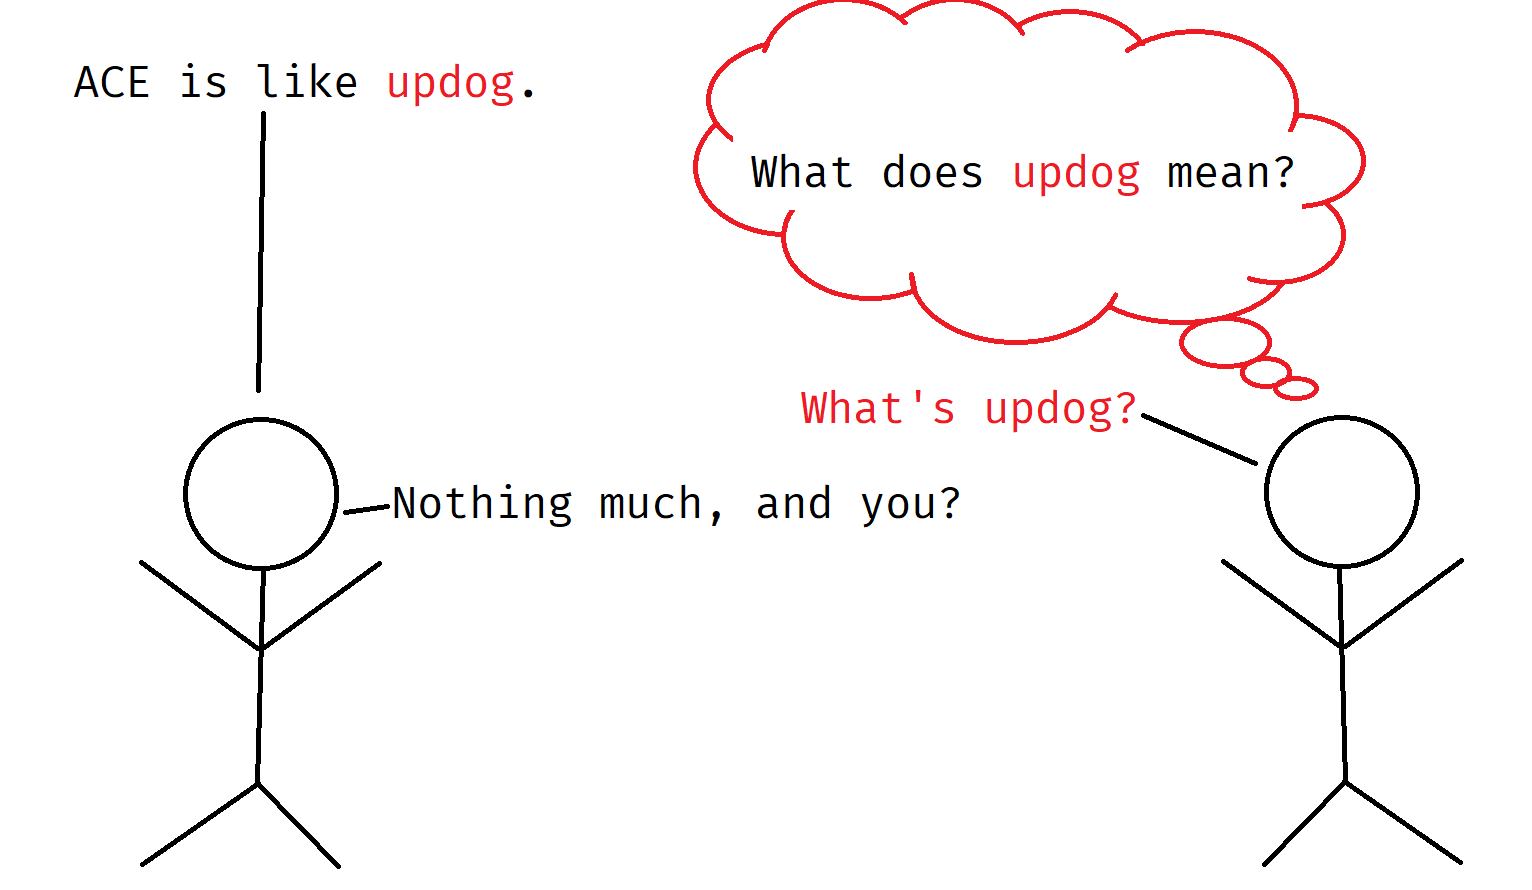
\includegraphics[scale=0.3]
		{figures/ace.png}}
	\caption{A graphical illustration of the \textit{updog} joke, credits to \href{https://www.youtube.com/watch?v=-XmXYCXX7y4}{Smoovers}}\label{fig:updog}
\end{figure}

This joke, illustrated in Figure \ref{fig:updog} is an extremely simple but direct way of explaining what ACE is. In this case the joke is self-explanatory, but the idea behind it is that we end up saying something (\textit{what's up dawg?}) that is not what we intended to say (\textit{what does updog mean?}). This is extremely similar to what happens during ACE in the real world (don't like this, gotta rephrase), where we end up executing code that we did not intend to execute, albeit with dramatically more complicated consequences.

To get a bit more into the proper definition of things: ACE is a type of flaw or vulnerability that allows an attacker to execute some (generally speaking) malicious code on a target system. Without proper protections and preventions put in place, an attacker can easily exploit these to gain access to sensitive information, take control of the system, or even cause damage to the system itself. The severity of this incidents can vary greatly: in the past these exploits have gone from allowing gamers to better their speedrunning performances (where speedrunning is the act of playing a video game with the goal of completing it as fast as possible), to leaking sensitive kernel memory on real world systems, as was the case in \href{https://comsec.ethz.ch/research/microarch/retbleed/}{Retbleed}.

These vulnerabilities can be exploited through various means, including buffer overflows, code injection, and other techniques; however in the context of this case study, we will be looking at a specific example of ACE in the world of video games, specifically in the game \textit{Pokémon Emerald} where the techniques used to exploit the vulnerabilities are \textbf{Arbitrary memory write} and \textbf{out-of-bounds writes}, which is where existing mechanics are used to place crafted instructions into writable areas.




\section{\textbf{Pokémon Emerald - case study}}
\subsection{\textbf{The Pomeg glitch}}
In Pokémon Emerald, the player can use a glitch called \textit{Pomeg glitch} to put the game in an impossible state. To explain this glitch first it would be wise to understand how the game roughly works. In Pokémon Emerald the player can be in two states: the exploration state, where they can go around the map with a team of up to six Pokémon which can be caught in, and the battle state, that is where the fighting happen. Any pokemon caught after the sixth gets sent in the PC which is a storage system that allows the player to store Pokémon that they do not want to carry with them. The Pokémon have their own stats, which improve based on their levels and what other Pokémon they fight. The statistic involved with the Pomeg glitch is \textit{HP} (Hit Points), which is the amount of health a Pokémon has. If a Pokémon's HP reaches 0, it faints and cannot be used until it is revived and if all of them reach 0, we get a game over and this can only happen when the game is in the battle state.

The HP statistic is calculated through the following formula:

\begin{equation}
	\text{HP} = \left( \frac{(2 \times \text{Base} + \text{IV} + \left( \frac{\text{EV}}{4} \right)) \times \text{Level}}{100} \right) + \text{Level} + 10
	\label{eq:ergodic_hypothesis}
\end{equation}

This formula gives us the maximum HP of a Pokémon, which is the maximum amount of health it can have. In the case of the \textit{pomeg glitch}, the only relevant variable is the EV value: this is because the EV value is the only statistic that can be directly modified based on the actions of the player. It is a number between 0 and 255, and it increases every time a Pokémon defeats another, but most importantly it can also be decreased by using certain items. In the case of the \textit{pomeg glitch}, the player can use a specific item called \textit{Pomeg berry} to lower the EV value of a Pokémon by 10. However, if, for example, the Pokémon's current HP was at 1, when updating the newly calculated HP statistic, both the current HP and max HP get lowered and as such, the game could set the current HP value to 0, or, even worse, something below it, like underflowing to $ 2^{16}-1$ or 65535 HP (due to the HP statistic being an unsigned two-bytes integer). Now, to use a \textit{Pomeg berry} the player needs to not be in the combat state, and this can create some issues because the game is only capable of handling game overs (which happens when all of the player's Pokémon reach 0 HP) if the player is in a combat state. The problem arises in the situation where the Pokémon whose HP is being updated is the only one with $HP > 1$, because the player may ends up with a party of only dead Pokémon, as can be seen in figure \ref{fig:dead_team}.

\begin{figure}[h!]
	\center{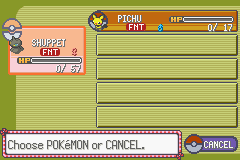
\includegraphics
		{figures/dead_team.png}}
	\caption{A technically impossible state}\label{fig:dead_team}
\end{figure}

This is not a problem at the second it happens, however if the player is to start a battle, the game will try to look for a Pokémon to fight with, and it will find none, because all of them are dead. So after unsuccessfully looking for a Pokémon to fight with, the game will then send out a \textbf{?} (commonly known in the Pokémon community as \textbf{Decamark}) as can be seen in Figure \ref{fig:decamark}, which is be used to prevent game crashes.

\begin{figure}[h!]
	\center{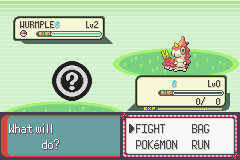
\includegraphics
		{figures/decamark.png}}
	\caption{The decamark Pokémon}\label{fig:decamark}
\end{figure}

At this point, the player can try to: fight, run away or use an item, all options which would result in a white out (the game over mechanic). But how can this lead to ACE? This is where the glitch known as \textit{Glitzer popping} comes into play.

\subsection{\textbf{Glitzer Popping}}
The \textit{Pomeg data corruption glitch}, most commonly known as the \textit{Glitzer popping}, is a glitch that allows the player to execute some arbitrary code by renaming the boxes to a specific string, which will then be interpreted as some code that will be executed when the game tries to read the name of the box. The player can rename the boxes to a specific string, obtaining different results spanning from obtaining event-exclusive items or Pokémon (for Pokémon Emerald many events were in-person at some specific locations), to modify player information or game flags, all the way to being able to execute custom scripts (like creating your own events). "But how do we get the game to read the name of the box to the point where it gets executed?" is the most logical follow-up question. The answer is simple: we need to use the \textit{Pomeg glitch}.


\subsubsection{\textbf{The setup}}
First things first, this thesis is not a tutorial on how to achieve this glitches, as there are countless fantastic other guides about replicating them (like \href{https://www.youtube.com/watch?v=45kwOEhKbUg}{this one}, or \href{https://e-sh4rk.github.io/ACE3/}{this one}), rather, my purpose is to illustrate and figure out why and how does ACE happen, using Pokémon Emerald as a basis for it.

To actually start executing some arbitrary code we need two things: the first one is the previously illustrated \textit{Pomeg glitch}, where the player is able to setup an impossible game state, and the second one needs the Boxes in which the Pokémon that don't fit in the player's team are stored. These are 14 different boxes in which the Pokémon are stored, and they can be renamed by the player. The names of these boxes are stored in a specific area of the memory, and this is where the player can start executing some code. The player can rename the boxes to a specific string, which will then be interpreted as some code that will be executed when the game tries to read the name of the box. This is where the \textit{Glitzer popping} comes into play: it is a technique that allows the player to execute some arbitrary code by renaming the boxes to a specific string, which will then be interpreted as some code that will be executed when the game tries to read the name of the box (an example can be seen in Table \ref{tab:boxes_names}).

\begin{table}[h!]
	\centering
	\begin{tabular}{|c|l|}
		\hline
		\textbf{Box} & \textbf{Name} \\
		\hline
		Box 1        & (VTTnFMBn)    \\
		Box 2        & (EEENJRo )    \\
		Box 3        & (EE5…Bq  )    \\
		Box 4        & (EFF…o   )    \\
		Box 5        & (KT?nTR?n)    \\
		Box 6        & (EEEIP?n )    \\
		Box 7        & (EE'FQm  )    \\
		Box 8        & (EmFlo   )    \\
		Box 9        & (yLRom"Ro)    \\
		Box 10       & (EEEFGEn )    \\
		Box 11       & (EE …?q  )    \\
		Box 12       & (E…P-n   )    \\
		Box 13       & (FQRn…TRn)    \\
		Box 14       & (EEEt ?n )    \\
		\hline
	\end{tabular}
	\caption{Example box names required to teleport to map ID \texttt{0B10}}
	\label{tab:boxes_names}
\end{table}


The game is not capable of handling the situation where the player has a Decamark in their team, and as such when the player tries to open their team information in battle it will unsuccessfully try to read the Pokémon's data from the memory, leaving instead a blank Pokémon.

% insert image here

So when the player moves the cursor to the first slot in their team, the cursor actually underflows and goes to slot 256  (since a team is made up of a maximum of 6 members) and as such, instead of scrolling through slots 1-6, we player has access to slots 255 and above (as the cursor is technically out of bounds). However, slots outside the first 6 aren't meant to be Pokémon slots, so the game accesses random blocks of RAM data and treats them as Pokémon, even though they are not. In this case the 255th party slot is actually the PC Pokémon data and continuing to scroll upwards allows the player to actually go over memory addresses reserved for various in-game data.

Each time the party Pokémon selection pointer moves to a new party slot, an anti-cheat verification routine is triggered for the selected "Pokémon" (because the game thinks it is, but it's actually not). If the checksum of the selected data block (interpreted as a Pokémon) is invalid, the game modifies it into a Bad Egg, which is the result of the anti-cheating protocol, a bad egg is what the game sees as a "cheated" or invalid Pokémon. This transformation involves setting the Egg Status flag to 1 and enabling two additional bits, which designate the Egg as a "Bad" Egg. Since the memory blocks being interpreted as party Pokémon are not genuine Pokémon structures, their checksums will almost always be invalid—unless the slot is empty.

The Egg Status flag can reside in one of four different locations within a Pokémon's data structure. It is part of one of the four substructures that make up a Pokémon which can be seen in \ref{fig:pokemon-data-structure}, and the order of these substructures is determined by the Pokémon's Personality Value (PID modulo 24). Because these substructures are encrypted using the Pokémon’s PID and the Trainer ID (TID), setting the Egg Status flag to 1 can result in either a bit value of 1 or 0, depending on the result of \texttt{PID} XOR \texttt{TID}. In contrast, the two bits that define a "Bad" Egg are always located at fixed positions, and they are consistently set to 1 when a checksum is invalid. These bit modifications are what cause memory corruption in RAM. However, since only three bits are affected within a block of 100 bytes, the resulting corruption is minimal. Additionally, one of the modified bits is not at a fixed location and may be toggled to either 1 or 0, introducing variability in both the location and nature of the corruption.

%%%%%%%%%%%%%%%%%%%%%%%%%%%%%%%%%%%%%%%%%%%%
%%%%%% TODO: Replace with actual table %%%%%
%%%%%%%%%%%%%%%%%%%%%%%%%%%%%%%%%%%%%%%%%%%%
\begin{figure}[h!]
	\center{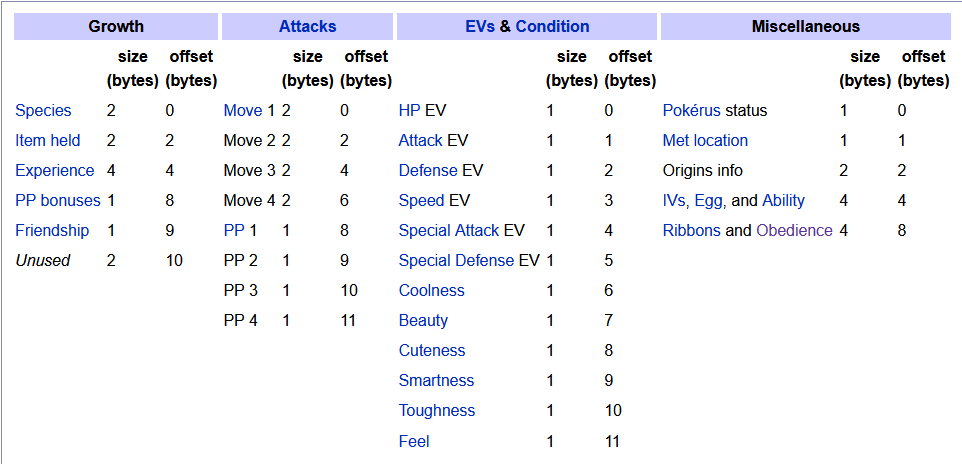
\includegraphics[width=\textwidth]
		{figures/sub-structure.png}}
	\caption{Pokémon Data Structure (by Substructure) credits to \href{https://bulbapedia.bulbagarden.net/wiki/Pokémon_data_substructures_(Generation_III)}{Bulbapedia}}
	\label{fig:pokemon-data-structure}
\end{figure}



An additional layer of randomness is introduced by the DMA (Direct Memory Access) system, which is another built-in anti-cheat mechanism that shifts the RAM addresses of numerous data structures whenever the player performs actions such as entering a battle, going through a doorway, or opening the Bag. The DMA remaps memory addresses using a translation table of multiple double-words. Any value subjected to DMA can occupy up to 32 different memory addresses, each spaced by 4 bytes (a double-word).

Importantly, party Pokémon are not affected by DMA, which means the memory addresses of the six standard party slots remain fixed. However, any data read from memory locations beyond the sixth slot \textit{is} subject to DMA. Since each party Pokémon occupies 25 double-words, and DMA remapping allows up to 32 double-word shifts, each double-word in a slot beyond the sixth could potentially be placed at an address susceptible to corruption via the Egg Status bit alterations. Due to the variability in both RAM content and corruption locations, these elements may interact unpredictably, sometimes preventing a given double-word from being corrupted by the Egg-related flags.





\subsubsection{\textbf{What actually goes on behind the scenes}}


\section{\textbf{State of the art chapter}}
\subsection{\textbf{What is the situation today}}


\subsection{\textbf{Current studies on security and improvements on protections}}




To insert a figure use the following command:

\begin{figure}[h!]
	\center{
\includegraphics[scale=0.03 ]
		{figures/flower.jpg}}
	\caption{The caption of my figure}\label{fig:flower}
\end{figure}




\section{\textbf{Conclusion}}
The experimental result goes here ... \footnote{https://www.usi.ch}. \\







\newpage
\section{\textbf{Future work}}

\section{\textbf{Summary}}
Future works goes here.






\newpage

%%%%% BIBLIOGRAPHY %%%%%
\bibliographystyle{abbrv}
\bibliography{references}

\end{document}
